% Submission Deadline: Thursday, 28 March 2013, 23:59 UTC-11 American Samoa time
%   = 21:59 PM Friday, 29 March 2013, Sydney
% Page limit: 12 pages

\documentclass{sigplanconf}
%\documentclass[preprint]{sigplanconf}

\usepackage{pdf14}
%\usepackage[british]{babel}
\usepackage{version}
\usepackage[pdftex]{graphicx}
\usepackage{amsmath}
\usepackage{amsfonts,amssymb}
\usepackage{url}
\usepackage{alltt}
\usepackage{code}
\usepackage{listings}
\usepackage{hyperref}
%\usepackage{doi}
\usepackage{haskell}
\usepackage{rotating}

% \renewcommand{\textfraction}{0.2}
% \renewcommand{\topfraction}{0.9}
% \renewcommand{\dbltopfraction}{0.9}
% \renewcommand{\floatpagefraction}{0.9}
% \renewcommand{\dblfloatpagefraction}{0.9}

\newcommand{\comm}[1]{$\langle$\textrm{#1}$\rangle$}
%\newcommand{\hscom}[1]{\textrm{\mbox{--- #1}}}

\newcommand{\note}[2]{\emph{\textbf{#1} #2}}

\newcommand{\app}{\ensuremath{\mathbin{\texttt{\char"40}}}}
\newcommand{\float}[3]{{#1}\stackrel{#2}{:}{#3}}
\hscommand{\letin}[2]{\mathtt{let} #1 \mathtt{in} #2}
 
\newcommand{\gck}[1]            {\note{GCK:}{#1}}
\newcommand{\manuel}[1]         {\note{MMTC:}{#1}}
\newcommand{\trev}[1]           {\note{TLM:}{#1}}
\newcommand{\ben}[1]            {\note{BL:}{#1}}
\newcommand{\TODO}[1]           {\note{TODO:}{#1}}
\newcommand{\finaltodo}[1]      {\note{TODO FINAL:}{#1}}
\newcommand{\REF}               {\note{REF}}
\newcommand{\CITE}              {\note{CITE}}

% listings
\lstloadlanguages{Haskell,C}
%\lstnewenvironment{code}[1][]
%    {\lstset{language=Haskell,#1}\csname lst@SetFirstLabel\endcsname}
%    {\csname lst@SaveFirstLabel\endcsname}
%
%\lstdefinestyle{inline}{frame=none,numbers=none,basicstyle=\footnotesize}

\lstset{
%    frame=single,
%    rulecolor={\color[gray]{0.7}},
%    numbers=left,
%    numberstyle=\tiny\it, %\color{Gray},
    commentstyle=\it, %\color{MidnightBlue},
    captionpos=b,
    xleftmargin=0.5\parindent,
    xrightmargin=0.5\parindent,
    %
    basicstyle=\ttfamily, %\scriptsize
    flexiblecolumns=false,
    basewidth={0.5em,0.45em},
%    literate=
%      {+}{{$+$}}1
%      {/}{{$/$}}1
%      {*}{{$*$}}1
%      {=}{{$=$}}1
%      {>}{{$>$}}1
%      {<}{{$<$}}1
%      {\\}{{$\lambda$}}1
%      {`}{{$\grave{}$}}1
%      {\\\\}{{\char`\\\char`\\}}1
%      {->}{{$\rightarrow$}}2
%      {>=}{{$\geq$}}2
%      {<-}{{$\leftarrow$}}2
%      {<=}{{$\leq$}}2
%      {=>}{{$\Rightarrow$}}2
%      {\ .}{{$\circ$}}2
%      {\ .\ }{{$\circ$}}2
%      {>>}{{>>}}2
%      {>>=}{{>>=}}2
%      {|}{{$\mid$}}1
}


% \makeatletter
% \def \ps@plain {%
%   \let \@mkboth = \@gobbletwo
%   \let \@evenhead = \@empty
%   \def \@evenfoot { \thepage \hfil \scriptsize \textit{\@preprintfooter}\hfil
%                    \textit{\@formatyear}}%
%   \let \@oddhead = \@empty
%   \let \@oddfoot = \@evenfoot}
% \makeatother

\begin{document}

\preprintfooter{\textbf{--- DRAFT --- DRAFT --- DRAFT --- DRAFT ---}}

\exclusivelicense
\conferenceinfo{ICFP~'13}{September 25--27, 2013, Boston, MA, USA}
\copyrightyear{2013}
\copyrightdata{978-1-4503-2326-0/13/09}
\doi{2500365.2500595}

\title{Optimising Purely Functional GPU Programs}
\authorinfo{
  Trevor L. McDonell \and
  Manuel M. T. Chakravarty \and
  Gabriele Keller \and
  Ben Lippmeier
  % \shortstack{%
  % }
}{
  University of New South Wales, Australia
}{
  \{tmcdonell,chak,keller,benl\}@cse.unsw.edu.au
}
\maketitle

\makeatactive

\begin{abstract}
Purely functional, embedded array programs are a good match for SIMD hardware, such as GPUs. However, the naive compilation of such programs quickly leads to both code explosion and an excessive use of intermediate data structures. The resulting slow-down is not acceptable on target hardware that is usually chosen to achieve high performance.
  
In this paper, we discuss two optimisation techniques, \emph{sharing recovery} and \emph{array fusion}, that tackle code explosion and eliminate superfluous intermediate structures. Both techniques are well known from other contexts, but they present unique challenges for an embedded language compiled for execution on a GPU. We present novel methods for implementing sharing recovery and array fusion, and demonstrate their effectiveness on a set of benchmarks.
\end{abstract}

\category{D.3.2}{Programming Languages}{Language Classification---Applicative (functional) languages; Concurrent, distributed, and parallel languages}
%\category{D.3.4}{Programming Languages}{Processors---Code generation}

%\terms Languages; Performance

\keywords Arrays; Data parallelism; Embedded language; Dynamic compilation; GPGPU; Haskell; Sharing recovery; Array fusion


% -----------------------------------------------------------------------------
%!TEX root = ../Main.tex
\section{Introdution}

The Haskell library ecosystem is blessed with a multitude of libraries for writing streaming data flow programs. Stand out examples include iteratee CITE, enumerator CITE, conduit CITE and pipes CITE. These libraries are based around ... and more recent examples such as pipes provide a useful set of algebraic equivalences that give a clean mathematical structure to the provided mathemetical structure.

Libraries such as iteratee and enumerator are typically used to deal with data sets that do not fit in main memory, as the constant space guarantee ensures that the program will run to completion without suffering an out-of-memory error. However, current computing platforms use multi-core processors, the programming models provided by such streaming libraries do not also provide a notion of \emph{parallelism} to help deal with the implied amount of data. They also lack support for branching data flows where produced streams can be consumed by several consumers without the programmer needing to had fuse them.

We provide several techniques that increase the scope of programs that can be written in such libraries. Our target applications concern \emph{medium data}, meaning data that is large enough that it does not fit in the main memory of a normal desktop machine, but not so large that we require a cluster of multiple physical machines. For a lesser amount of data one could simply load the data into main memory and use an in-memory array library such as CITE or CITE. For greater data one needs to turn to a distributed system such as Hadoop or Spark and deal with the unreliable network and lack of shared memory. Repa Flow targets the sweet middle ground.

We make the following contributions:

\begin{itemize}
\item Our parallel data flows consist of a bundle of streams, where each stream can process a separate partition of a data set on a separate processor core.

\item Our API uses polarised flow endpoints (@Sources@ and @Sinks@) to ensure that programs run in constant space. We demonstrate how this standard technique can be extended to branching data flows, where produced flows are consumed by multiple consumers.

\item The data processed by our streams is chunked so that each operation processes several elements at a time. We show how to design the core API in a generic fashion so that chunk-at-a-time operators can interoperate smoothly with element-at-a-time operators.
\TODO{We don't support leftovers}

\item We show how to use Continuation Passing Style to provoke the Glasgow Haskell Compiler into applying stream fusion across chunks processed by independent flow operators. For example, the map-map fusion on flows arises naturally from map-map fusion rule on chunks (arrays) of elements.
\end{itemize}

Our work is embodied in Repa Flow, which is available on Hackage. \TODO{Specify the relationship to previous work on Repa}. This is a new layer on the original delayed arrays of our original Repa library.


%!TEX root = ../acc-optim.tex
\section{Optimising embedded array code} % (fold)
\label{sec:example}

\emph{Accelerate} is a \emph{domain specific} language, consisting of a carefully selected set of array operators that we can produce efficient GPU code for. Accelerate is \emph{embedded} in Haskell, meaning that we write Accelerate programs using Haskell syntax, but do not compile arbitrary Haskell programs to GPU machine code. Accelerate is stratified into \emph{array computations}, wrapped in a type constructor @Acc@, and \emph{scalar expressions}, represented by terms of type @Exp t@, where @t@ is the type of value produced by the expression. This stratification is necessary due to the hardware architecture of GPUs and their reliance on SIMD parallelism, as we discussed in our previous work~\cite{Chakravarty:Accelerate}.


% -----------------------------------------------------------------------------
\subsection{Too many kernels}
\label{code:dotp}

For example, to compute a dot product, we use:
%
\begin{quote}
\begin{code}
dotp :: Vector Float -> Vector Float 
     -> Acc (Scalar Float)
dotp xs ys = let xs' = use xs
                 ys' = use ys
             in  fold (+) 0 (zipWith (*) xs' ys')
\end{code}
\end{quote}
%
The function @dotp@ consumes two one-dimensional arrays (@Vector@) of floating-point values and produces a single (@Scalar@) floating-point result. From the return type @Acc (Scalar Float)@, we see that @dotp@ is an embedded Accelerate computation, rather than vanilla Haskell code.

The functions @zipWith@ and @fold@ are defined in our library @Data.Array.Accelerate@, and have \emph{massively parallel} GPU implementations with the following type signatures:
%
\begin{quote}
\begin{code}
zipWith :: (Shape sh, Elt a, Elt b, Elt c)
        => (Exp a -> Exp b -> Exp c)
        -> Acc (Array sh a) 
        -> Acc (Array sh b) 
        -> Acc (Array sh c)

fold    :: (Shape ix, Elt a)
        => (Exp a -> Exp a -> Exp a)
        -> Exp a
        -> Acc (Array (ix:.Int) a)
        -> Acc (Array ix a)
\end{code}
\end{quote}
%
The type classes @Elt@ and @Shape@ indicate that a type is admissible as an array element and array shape, respectively. Array shapes are denoted by type-level lists formed from @Z@ and @(:.)@ --- for example, @Z:.Int:.Int@ is the shape of a two-dimensional array (see \cite{Keller:Repa,Chakravarty:Accelerate} for details). The type signatures of @zipWith@ and @fold@ clearly show the stratification into scalar computations using the @Exp@ type constructor, and array computations wrapped in @Acc@.

The arguments to @dotp@ are of plain Haskell type @Vector Float@. To make these arguments available to the Accelerate computation they must be embedded with the @use@ function:
%
\begin{quote}
\begin{code}
use :: Arrays arrays => arrays -> Acc arrays
\end{code}
\end{quote}
%
This function is overloaded so that it can accept entire tuples of @arrays@. Operationally, @use@ copies array data from main memory to GPU memory, in preparation for processing by the GPU.

The above Haskell version of the GPU-accelerated dot product is certainly more compact than the corresponding CUDA C code. However, when compiled with the skeleton-based approach we described in previous work~\cite{Chakravarty:Accelerate}, it is also significantly slower. The CUDA C version executes in about half the time (see Table~\ref{tab:benchmark-summary}).

The slow-down is due to Accelerate generating one \emph{GPU kernel function} for @zipWith@ and another one for @fold@. In contrast, the CUDA C version only uses a single kernel. The use of two separate kernels requires an intermediate array to be constructed, and in a memory bound benchmark, such as @dotp@, this doubles the runtime. To eliminate this intermediate array we need to \emph{fuse} the adjacent aggregate array computations. Although there is an existing body of work on array fusion, no existing method adequately deals with massively parallel GPU kernels. We present a suitable fusion framework as the first major contribution of this paper.


% -----------------------------------------------------------------------------
\subsection{Too little sharing}

As a second example, consider the pricing of European-style options using the Black-Scholes formula. The Accelerate program is in Figure~\ref{fig:black-scholes}.
%
\begin{figure*}
\hspace*{-2ex}\begin{minipage}{.55\textwidth}
\begin{code}
blackscholes :: Vector (Float, Float, Float) 
             -> Acc (Vector (Float, Float))
blackscholes = map callput . use
  where
  callput x =
    let (price, strike, years) = unlift x
        r       = constant riskfree
        v       = constant volatility
        v_sqrtT = v * sqrt years
        d1      = (log (price / strike) + 
                  (r + 0.5 * v * v) * years) / v_sqrtT
        d2      = d1 - v_sqrtT
        cnd d   = let c = cnd' d in d >* 0 ? (1.0 - c, c)
        cndD1   = cnd d1
        cndD2   = cnd d2
        x_expRT = strike * exp (-r * years)
    in
    lift ( price * cndD1 - x_expRT * cndD2
         , x_expRT * (1.0 - cndD2) - price * (1.0 - cndD1))
\end{code}
\end{minipage}
\begin{minipage}{.5\textwidth}
\begin{code}
riskfree, volatility :: Float
riskfree   = 0.02
volatility = 0.30

horner :: Num a => [a] -> a -> a
horner coeff x = x * foldr1 madd coeff
  where
    madd a b = a + x*b

cnd' :: Floating a => a -> a
cnd' d =
  let poly     = horner coeff
      coeff    = [0.31938153, -0.356563782, 
                  1.781477937, -1.821255978, 
                  1.330274429]
      rsqrt2pi = 0.39894228040143267793994605993438
      k        = 1.0 / (1.0 + 0.2316419 * abs d)
  in
  rsqrt2pi * exp (-0.5*d*d) * poly k
\end{code}
\end{minipage}
  \caption{Black-Scholes option pricing in Accelerate}
  \label{fig:black-scholes}
\end{figure*}
%
Given a vector of triples of underlying stock price, strike price, and time to maturity (in years), the Black-Scholes formula computes the price of a call and a put option. The function @callput@ evaluates the Black-Scholes formula for a single triple, and @blackscholes@ maps it over a vector of triples, such that all individual applications of the formula are executed in parallel.

If we compare the performance of the GPU code generated by Accelerate with that of an equivalent implementation in CUDA C, the Accelerate version is almost twenty times slower. As @blackscholes@ includes only one aggregate array computation, the problem can't be a lack of fusion. Instead, as we noted previously~\cite{Chakravarty:Accelerate}, it is due to the embedding of Accelerate in Haskell.

The function @callput@ includes a significant amount of sharing: the helper functions @cnd'@, and hence also @horner@, are used twice ---for @d1@ and @d2@--- and its argument @d@ is used multiple times in the body. Our embedded implementation of Accelerate reifies the abstract syntax of the (deeply) embedded language in Haskell. Consequently, each occurrence of a let-bound variable in the source program creates a separate unfolding of the bound expression in the compiled code.

This is a well known problem that has been solved elegantly by the \emph{sharing recovery} algorithm of \citet{Gill:2009dx}, which makes use of stable names. Unfortunately, Gill's original approach (1) reifies the abstract syntax in \emph{graph} form and (2) it assumes an \emph{untyped} syntax representation. In contrast, Accelerate is based on a typed tree representation using GADTs and type families in conjunction with type-preserving compilation in most phases. In other words, we use Haskell's type checker to statically ensure many core properties of our Accelerate compiler. The fact that the compiler for the \emph{embedded language} is type preserving, means that many bugs in the Accelerate compiler itself are caught by the Haskell compiler during development. This in turn reduces the number of Accelerate compiler bugs that the end-user might be exposed to.

As we require typed trees, where sharing is represented by let bindings rather than untyped graphs, we cannot directly use Gill's approach to sharing recovery. Instead, we have developed a novel sharing recovery algorithm, which like Gill's, uses stable names, but unlike Gill's, operates on typed abstract syntax. Our algorithm produces a typed abstract syntax \emph{tree}, and we are able to recover exactly those let bindings used in the source program. This is the second major contribution of this paper.


% -----------------------------------------------------------------------------
\subsection{Summary}
In summary, a straightforward skeleton-based implementation of an embedded GPU language suffers from two major inefficiencies: \emph{lack of sharing} and \emph{lack of fusion.} Both sharing recovery in embedded languages, and array fusion in functional languages have received significant prior attention. However, we have found that none of the existing techniques are adequate for a \emph{type-preserving} embedded language compiler targeting \emph{massively parallel SIMD hardware,} such as GPUs.

% section example (end)

%!TEX root = ../acc-optim.tex
\section{Sharing recovery} % (fold)
\label{sec:sharing}

% It turns out that Emil Axelsson's Syntactic library implements typed sharing recovery using
% graphs as proposed by Gill. This is based on a graph version of Syntactic's extensible ASTs
% (and not explained in Axelsson's 2012 ICFP paper). Syntactic supports converting a graph
% with sharing backend into a tree, but it doesn't seem to support generating a let-based
% representation.
%
% How does the type safety work out in the graph representation? Are transformations really
% properly typed? 
%
% Axelsson's implementation of sharing recovery is less functional than ours. The whole process
% is in IO and, in addition to stable names, also makes use of 'IORef's.
%
% The implementation was committed July 2011: 
%   http://hub.darcs.net/emax/syntactic/patch/20110719132827-080f5
% We implemented the current version of sharing recovery in early to mid 2011 (and a preliminary
% version end of 2010).

\citet{Gill:2009dx} proposed to use \emph{stable names}~\cite{PeytonJones:StorageManager} to recover the sharing of source terms in a deeply embedded language. The stable names of two Haskell terms are equal only when the terms are represented by the same heap structure in memory. Likewise, when the abstract syntax trees (ASTs) of two terms of an embedded language have the same stable name, we know that they represent the same value. In this case we should combine them into one shared AST node. As the stable name of an expression is an intensional property, it can only be determined in Haskell's @IO@ monad.

Accelerate's runtime compiler preserves source types throughout most of the compilation process~\cite{Chakravarty:Accelerate}. In particular, it converts the source representation based on higher-order abstract syntax (HOAS) to a type-safe internal representation based on de Bruijn indices. Although developed independently, this conversion is like the \emph{unembedding} of \citet{Atkey:Unembedding}. Unembedding and sharing recovery necessarily need to go hand in hand for the following reasons. Sharing recovery must be performed on the source representation; otherwise, sharing will already have been lost. Nevertheless, we cannot perform sharing recovery on higher-order syntax as we need to traverse below the lambda abstractions used in the higher-order syntax representation. Hence, both need to go hand in hand.

As shown by \citet{Atkey:Unembedding}, the conversion of HOAS in Haskell can be implemented in a type-preserving manner with the exception of one untyped, but dynamically checked environment look up, using Haskell's @Typeable@. To preserve maximum type safety, we do not want any further operations that are not type preserving when adding sharing recovery. Hence, we cannot use Gill's algorithm. The variant of Gill's algorithm used in Syntactic~\cite{Axelsson:Syntactic} does not apply either: it (1) also generates a graph and (2) discards static type information in the process. In contrast, our novel algorithm performs simultaneous sharing recovery and conversion from HOAS to a typed de Bruijn representation, where the result of the conversion is a tree (not a graph) with sharing represented by let bindings. Moreover, it is a type-preserving conversion whose only dynamically checked operation is the same environment lookup deemed unavoidable by \citet{Atkey:Unembedding}.

In the following, we describe our algorithm using plain typed lambda terms. This avoids much of the clutter that we would incur by basing the discussion on the full Accelerate language. In addition to its implementation in Accelerate, a working Haskell implementation of our algorithm for the plain lambda calculus can be found at \url{https://github.com/mchakravarty/hoas-conv}.


% -----------------------------------------------------------------------------
\subsection{Our approach to sharing recovery}

\begin{figure*}
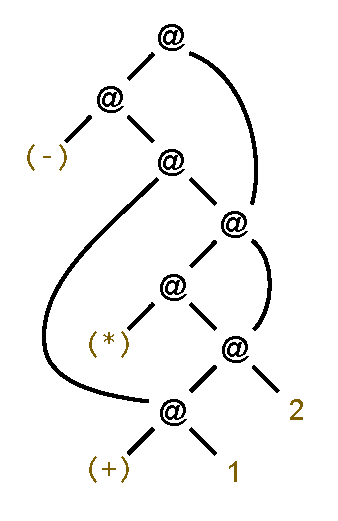
\includegraphics[scale=0.6]{figs/sharing-original.pdf}
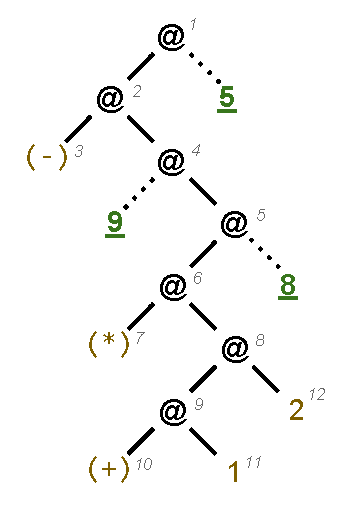
\includegraphics[scale=0.6]{figs/sharing-pruned.pdf}
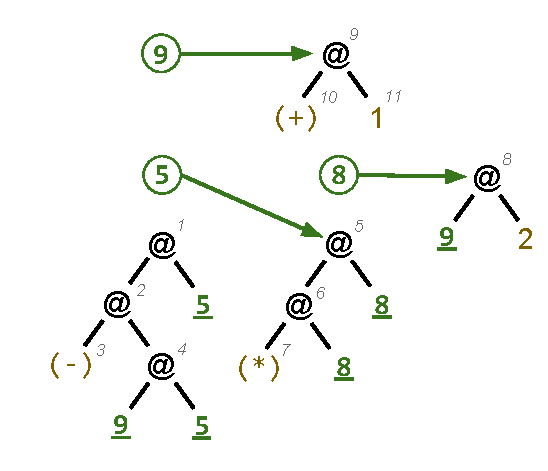
\includegraphics[scale=0.6]{figs/sharing-floated.pdf}
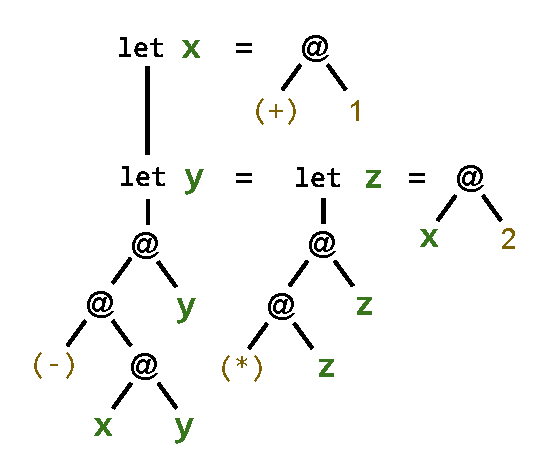
\includegraphics[scale=0.6]{figs/sharing-lets.pdf}
\caption{Recovering sharing in an example term}
\label{fig:sharing}
\end{figure*}
%
Before we formalise our sharing recovery algorithm in the following subsections, we shall illustrate the main idea. Consider the following source term:
%
\begin{quote}
\begin{code}
let    inc  = (+) 1
in let nine = let three = inc 2 
              in
              (*) three three
in
(-) (inc nine) nine
\end{code}
\end{quote}
%
This term's abstract syntax DAG is the leftmost diagram in Figure~\ref{fig:sharing}. It uses \app\ nodes to represent applications; as in this grammar:%
%
\begin{haskell*}
  T &{}\to{}& C 
  &\qquad& T^\tau \mathbf{where}\\
    &\mid   & x 
  &      &~~~C^\tau &:: T^\tau\\
    &\mid   & \lambda{x}. T 
  &      &~~~x^\tau &:: T^\tau\\
    &\mid   & T_1\app{}T_2
  &      &~~~\lambda{x^{\tau_1}}.T^{\tau_2} &:: T^{\tau_1\to\tau_2}\\
  C &\to    & \langle\text{constants}\rangle
  &      &~~~T_1^{\tau_1\to\tau_2}\app{}T_2^{\tau_1} &:: T^{\tau_2}
\end{haskell*}
%
The left definition does not track types, whereas the right one does. We implement typed ASTs in Haskell with GADTs and work with typed representations henceforth. Typed HOAS conversion with sharing recover proceeds in three stages:
%
\begin{enumerate}
  \item \emph{Prune shared subterms:} A depth first traversal over the AST annotates each node with its unique stable name, where we build an occurrence map of how many times we've already visited each node. If we encounter a previously visited node, it represents a \emph{shared subterm}, and we replace it by a placeholder containing its stable name. The second diagram in Figure~\ref{fig:sharing} shows the outcome of this stage. Each node is labeled by a number that represents its stable name, and the dotted edges indicate where we encountered a previously visited, shared node. The placeholders are indicated by underlined stable names.
  
  \item \emph{Float shared terms:} All shared subterms float upwards in the tree to just above the lowest node that dominates all edges to the original position of that shared subterm --- see the third diagram in Figure~\ref{fig:sharing}. Floated subterms are referenced by circled stable names located \emph{above} the node that they floated to. If a node collects more than one shared subterm, the subterm whose origin is deeper in the original term goes on top --- here, 9 on top of 5. Nested sharing leads to subterms floating up inside other floated subterms --- here, 8 stays inside the subterm rooted in 5.

  \item \emph{Binder introduction:} Each floated subterm gets let-bound right above the node it floated to (rightmost diagram in Figure~\ref{fig:sharing}). While we use explicit, bound names in the figure, we introduce de Bruijn indices at the same time as introducing the lets. 
\end{enumerate}


% -----------------------------------------------------------------------------
\subsection{Prune shared subterms}

First, we identify and prune shared subtrees, producing a pruned tree of the following form (second diagram in Figure~\ref{fig:sharing}):
%
\newcommand{\cT}{{^{\circ}\!T}}
\begin{haskell}
  \cT^\tau \mathbf{where} \\
  ~~~~\ell               &:: \cT^\tau
          &~& \hscom{binder conversion level}\\
  ~~~~\underline\nu^\tau  &:: \cT^\tau
          &~& \hscom{pruned subtree (name)}\\
  ~~~~C^\tau              &:: \cT^\tau \\
  ~~~~\lambda\ell.\cT^{\tau_2} &:: \cT^{\tau_1\to\tau_2} \\
  ~~~~\cT_1^{\tau_1\to\tau_2}\app{}\cT_2^{\tau_1} &:: \cT^{\tau_2} \\
\end{haskell}
% \begin{haskell*}
%   T^\circ &{}\to{}& \ell 
%           &~& \hscom{level for HOAS to de Buijn conversion}\\
%           &\mid   & \underline\nu
%           &~& \hscom{stable name of pruned shared subtree}\\
%           &\mid   & C \\
%           &\mid   & \lambda\ell. T^\circ \\
%           &\mid   & T_1^\circ\app{}T_2^\circ \\
% \end{haskell*}
%

A stable name (here, of type \<Name\>) associates a unique name with each unique term node, so that two terms with the same stable name are identical, and are represented by the same data structure in memory. Here, we denote the stable name of a term as a superscript during pattern matching --- e.g., \(1^\nu\) is a constant with stable name $\nu$, just as in the second and third diagram in Figure~\ref{fig:sharing}.

An \emph{occurrence map}, \<\Omega :: Name \mapsto Int\>, is a finite map that determines the number of occurrences of a $\textit{Name}$ that we encountered during a traversal. The expression \(\Omega\nu\) yields the number of occurrences of the name $\nu$, and we have \mbox{\(\nu\in\Omega \equiv (\Omega\nu > 0)\)}. To add an occurrence to $\Omega$, we write \(\nu\rhd\Omega\). We will see in the next subsection that we cannot simplify $\Omega$ to be merely a set of occurring names. We need the actual occurrence count to determine where shared subterms should be let-bound.

The identification and pruning of shared subtrees is formalised by the following function operating on \emph{closed} terms from \<T^\tau\>:
%
\bgroup
\hsmargin0pt
\begin{haskell}
  \hsnoalign{prune :: Level \to (Name \mapsto Int) \to T^\tau \to ((Name \mapsto Int), \cT^\tau)}
  prune \ell \Omega e^\nu &\mid \nu\in\Omega &= (\nu\rhd\Omega, \underline\nu) \\
  prune \ell \Omega e^\nu &\mid otherwise    &= enter (\nu\rhd\Omega) e
  \hswhere{
    enter \Omega c                &= (\Omega, c) \\
    enter \Omega (\lambda{x}.e)   &= \hslet{(\Omega', e') = prune (\ell+1) \Omega ([\ell/x]e)}{(\Omega', \lambda\ell.e')} \\
    enter \Omega ({e_1}\app{e_2}) &= 
      \hslet{
          (\Omega_1, e_1') = prune \ell \Omega e_1 \\
          (\Omega_2, e_2') = prune \ell \Omega_1 e_2
        }{
          (\Omega_2, {e_1'}\app{e_2'})
        } \\
  }
\end{haskell}
\egroup
%
% \ben{We can't perform the substitution $[\ell/x]e$ because while $e$ has type $T$, $\ell$ has type $\cT$. We'd instead need to keep a map of $Vars \mapsto Levels$ and update this on the way down.}
% As this is HOAS, we cannot have a map of $Vars \mapsto Levels$ either. Instead, we have $\ell$ already in $T$ in the Haskell implementation. Even more precisely, we don't have $[\ell/x]e$, but the $\lambda$ is a really Haskell function and we apply it to $\ell$. Doing this exactly as in Haskell would add clutter and additional explanation. As we are doing the morally right thing here, I think, it is ok to leave it as it is.
%
The first equation of \<prune\> covers the case of a term's repeated occurrence. In that case, we prune sharing by replacing the term \<e^\nu\> by a tag \<\underline\nu\> containing its stable name --- these are the dotted lines in the second diagram in Figure~\ref{fig:sharing}.

To interleave sharing recovery with the conversion from HOAS to typed de Bruijn indices, \<prune\> tracks the nesting \<Level\> of lambdas. Moreover, the lambda case of \<enter\> replaces the HOAS binder \<x\> by the level \<\ell\> at the binding and usage sites.

Why don't we separate computing occurrences from tree pruning? When computing occurrences, we must not traverse shared subtrees multiple times, so we can as well prune at the same time. Moreover, in the first line of \<prune\>, we cannot simply return \<e\> instead of \<\underline\nu\> --- \<e\> is of the wrong form as it has type \<T\> and not \<\cT\>! 

As far as type-preservation is concerned, we do lose information due to replacing variables by levels $\ell$. This is the inevitable loss described by \citet{Atkey:Unembedding}, which we make up for by a dynamic check in an environment lookup, as already discussed.

% We could not enter shared subtrees multiple times and still leave pruning to the following stage. This has some advantages and some disadvantages (need to use the occurrences map in the next round again to spot shared subtrees). There seems to be no one undisputedly best decomposition here.


% -----------------------------------------------------------------------------
\subsection{Float shared subterms}

Second, we float all shared subtrees out to where they should be let-bound, represented by (see third diagram in Figure~\ref{fig:sharing})
%
\newcommand{\uT}{{^\uparrow\!T}}
\newcommand{\dT}{{^\downarrow\!T}}
\begin{haskell}
  \hsnoalign{\uT^\tau {}\to{} \overline{\nu : \uT^{\tau'}} \succ \dT^\tau}
  \dT^\tau \mathbf{where} \\
  ~~~~\underline\nu^\tau  &:: \dT^\tau \\
  ~~~~C^\tau              &:: \dT^\tau \\
  ~~~~\lambda\nu.\uT^{\tau_2} &:: \dT^{\tau_1\to\tau_2} \\
  ~~~~\uT_1^{\tau_1\to\tau_2}\app{}\uT_2^{\tau_1} &:: \dT^{\tau_2} \\
\end{haskell}
% \begin{haskell*}
%   T^\uparrow &{}\to{}& \overline{\nu : T^\uparrow} \succ T^\downarrow \\
%   T^\downarrow
%           &{}\to{}& \underline\nu \\
%           &\mid   & C \\
%           &\mid   & \lambda\nu. T^\uparrow \\
%           &\mid   & T_1^\uparrow\app{}T_2^\uparrow \\
% \end{haskell*}
%
A term in \<\uT\> comprises a sequence of floated-out subterms labelled by their stable name as well as a body term from \<\dT\> from which the floated subterms where extracted. Moreover, the levels \<\ell\> that replaced lambda binders in \<\cT\> get replaced by the stable name of their term node. This simplifies a uniform introduction of de Bruijn indices for let and lambda bound variables. 

We write \<\overline{\nu : \uT}\> for a possibly empty sequence of items: \<\nu_1 : \uT_1, \ldots, \nu_n : \uT_n\>, where $\bullet$ denotes an empty sequence. 
%When the sequence of floated subterms is empty we sometimes write just \<T^\downarrow\> as shorthand for \<{\bullet}\succ{T^\downarrow}\>.
% Really? Where?

The floating function \<float\> maintains an auxiliary structure of floating terms and levels, defined as follows:
%
% \begin{haskell*}
%   \Gamma &{}\to{}& \float\nu{i}{T^\uparrow} &~&\hscom{floated shared subtree} \\
%          &\mid   & \float\nu{i}\cdot        &~&\hscom{floated pruned subtree} \\
%          &\mid   & \float\nu{i}\ell         &~&\hscom{floated level tag} \\
% \end{haskell*}
\begin{haskell*}
  \Gamma &{}\to{}& \float\nu{i}{\uT^\tau} 
          {}\mid{} \float\nu{i}\cdot
          {}\mid{} \float\nu{i}\ell
\end{haskell*}
%
These are floated subtrees named \<\nu\> of which we have collected $i$ occurrences. The occurrence count indicates where a shared subterm gets let bound: namely at the node where it matches \<\Omega\nu\>. This is why \<prune\> needed to collect the number of occurrences in \<\Omega\>. When the occurrence count matches \<\Omega\nu\>, we call the floated term \emph{saturated}. The following function determines saturated floated terms, which ought to be let bound:
%
\begin{haskell}
  \hsnoalign{bind :: (Name \mapsto Int) \to \overline\Gamma \to \overline{\exists\tau.\nu : \uT^\tau}}
  bind \Omega \bullet                             &= \bullet \\
  bind \Omega (\float\nu{i}e, \overline\Gamma)
    \mid \Omega\nu == i                           &= \nu:e, bind \Omega \overline\Gamma \\
  bind \Omega (\float\nu{i}\_, \overline\Gamma)   &= bind \Omega \overline\Gamma
\end{haskell}
%
Note that \<\Gamma\> does not keep track of the type \<\tau\> of a floated term \<\uT^\tau\>; hence, floated terms from \<bind\> come in an existential package. This does \emph{not} introduce additional loss of type safety as we already lost the type of lambda bound variables in \<\float\nu{i}\ell\>. It merely means that let bound, just like lambda bound, variables require the dynamically checked environment look up we already discussed.

When floating the \emph{first occurrence} of a shared tree (not pruned by \<prune\>), we use \<\float\nu{i}{\uT^\tau}\>. When  floating \emph{subsequent occurrences} (which were pruned), we use \<\float\nu{i}\cdot\>. Finally, when floating a level, to replace it by a stable name, we use \<\float\nu{i}\ell\>.

We define a partial ordering on floated terms: \<\float{\nu_1}{i}{x} < \float{\nu_2}{j}{y}\> iff the direct path from \<\nu_1\> to the root of the AST is shorter than that of \<\nu_2\>. We keep sequences of floated terms in \emph{descending order} --- so that the deepest subterm comes first. We write \<\overline{\Gamma_1}\uplus\overline{\Gamma_2}\> to merge two sequences of floated terms. Merging respects the partial order, and it combines floated trees with the same stable name by adding their occurrence counts. To combine the first occurrence and a subsequent occurrence of a shared tree, we preserve the term of the first occurrence. We write \<\overline\Gamma\setminus\overline\nu\> to delete elements of \<\overline\Gamma\> that are tagged with a name that appears in the sequence \<\overline\nu\>.

We can now formalise the floating process as follows:
%
\begin{haskell}
  \hsnoalign{float :: (Name \mapsto Int) \to \cT^\tau \to (\overline\Gamma, \uT^\tau)}
  float \Omega \ell^\nu      &= (\float\nu{1}\ell,  \underline\nu)\\
  float \Omega \underline\nu &= (\float\nu{1}\cdot, \underline\nu)\\
  float \Omega e^\nu         &= 
  \hslet{
    (\overline\Gamma, e')    &= descend e \\
    \overline{\nu_b : e_b}   &= bind \Omega \overline\Gamma \\
    d                        &= \overline{\nu_b : e_b} \succ e'
  }{%
    \hsif{
      \Omega\nu == 1
    }{
      (\overline\Gamma\setminus\overline{\nu_b}, d)  
    }{
      \hsalign{
        (\overline\Gamma\setminus\overline{\nu_b}\uplus\{\nu:d\}, \underline\nu)
      }
    }
  }
  \hswhere{
    \hsnoalign{descend :: \cT^\tau \to (\overline\Gamma, \dT^\tau)}
    descend c               &= (\bullet, c)\\
    descend (\lambda\ell.e) &= 
      \hslet{
        (\overline\Gamma, e') = float \Omega e
      }{
        \hsif{
          \exists \nu' i. (\float{\nu'}{i}\ell)\in\overline\Gamma
        }{
          (\overline\Gamma\setminus\{\nu'\}, \lambda\nu'.e')
        }{
          (\overline\Gamma, \lambda\_.e')
        }
      }\\
    descend ({e_1}\app{e_2}) &= 
      \hslet{
        (\overline\Gamma_1, e_1') = float \Omega e_1 \\
        (\overline\Gamma_2, e_2') = float \Omega e_2
      }{
        (\overline\Gamma_1\uplus\overline\Gamma_2, {e_1'}\app{e_2'})
      }
  }
\end{haskell}
%
The first two cases of \<float\> ensure that the levels of lambda bound variables and the names of pruned shared subterms are floated regardless of how often they occur. In contrast, the third equation floats a term with name $\nu$ only if it is shared; i.e., \<\Omega\nu\> is not 1. If it is shared, it is also pruned; i.e., replaced by its name \<\underline\nu\> --- just as in the third diagram of Figure~\ref{fig:sharing}.

Regardless of whether a term gets floated, all saturated floated terms, \<\overline{\nu_b : e_b}\>, must prefix the result, \<e'\>, and be removed from \<\overline\Gamma\>.

When \<descend\>ing into a term, the only interesting case is for lambdas. For a lambda at level \<\ell\>, we look for a floated level of the form \<\nu':\ell\>. If that is available, \<\nu'\> replaces \<\ell\> as a binder and we remove \<\nu':\ell\> from \<\overline\Gamma\>. However, if \<\nu':\ell\> is not in \<\overline\Gamma\>, the binder introduced by the lambda doesn't get used in \<e\>. In this case, we pick an arbitrary new name; here symbolised by an underscore ''\<\_\>''.


% -----------------------------------------------------------------------------
\subsection{Binder introduction}

Thirdly, we introduce typed de Bruijn indices to represent lambda and let binding structure (rightmost diagram in Figure~\ref{fig:sharing}):
%
\newcommand{\iT}[1][env]{{^{#1}\!T}}
\newcommand{\idx}[1][env]{{^{#1}\!\iota}}
\begin{haskell}
  \iT^\tau \mathbf{where} \\
  ~~~~C^\tau              &:: \iT^\tau \\
  ~~~~\idx^\tau           &:: \iT^\tau \\
  ~~~~\lambda{\iT[(\tau_1, env)]^{\tau_2}} &:: \iT^{\tau_1\to\tau_2} \\
  ~~~~\iT_1^{\tau_1\to\tau_2}\app{}\iT_2^{\tau_1} &:: \iT^{\tau_2} \\
  ~~~~\letin{\iT_1^{\tau_1}}{\iT[(\tau_1, env)]_2^{\tau_2}} &:: \iT^{\tau_2} \\
\end{haskell}
% \begin{haskell*}
%   T^\iota &{}\to{}& C \\
%           &\mid   & \iota \\
%           &\mid   & \lambda{T^\iota} \\
%           &\mid   & T_1^\iota\app{}T_2^\iota \\
%           &\mid   & \letin{T_1^\iota}{T_2^\iota} \\
% \end{haskell*}
%
With this type of terms, \<e::\iT^\tau\> means that \<e\> is a term representing a computation producing a value of type \<\tau\> under the type environment \<env\>. Type environments are nested pair types, possibly terminated by a unit type \<()\>. For example, \<(((), \tau_1), \tau_0)\> is a type environment, where de Bruijn index 0 represents a variable of type \<\tau_0\> and de Bruijn index 1 represents a variable of type \<\tau_1\>.

We abbreviate \<\mathtt{let} e_1 \mathtt{in} \cdots \mathtt{let} e_n \mathtt{in} e_b\> as \<\letin{\overline{e}}{e_b}\>. Both \<\lambda\> and \<\mathtt{let}\> use de Bruijn indices \<\iota\> instead of introducing explicit binders.

To replace the names of pruned subtrees and of lambda bound variables by de Bruijn indices, we need to construct a suitable type environment as well as an association of environment entries, their de Bruijn indices, and the stable names that they replace. We maintain the type environment with associated de Bruijn indices in the following \emph{environment layout} structure:
%
\newcommand{\Lyt}[1][env]{{^{#1}\!\Delta}}
\begin{haskell}
  \Lyt^{env'} \hskwd{where} \\
  ~~~~\circ &:: \Lyt^{()} \\
  ~~~~\Lyt^{env'};\idx^\tau &:: \Lyt^{(env', t)} \\
\end{haskell}
%
Together with a layout, we use a sequence of names \<\overline\nu\> of the same size as the layout, where corresponding entries represent the same variable. As this association between typed layout and untyped sequence of names is not validated by types, the lookup function \<lyt\mathrel\downarrow{i}\> getting the $i$th index of layout \<lyt\> makes use of a dynamic type check. It's signature is \<(\downarrow) :: \mathbb{N} \to \Lyt^{env'} \to \idx^\tau\>.

Now we can introduces de Bruijn indices to body expressions:
%
\begin{haskell}
  \hsnoalign{body :: \Lyt^{env} \to \overline\nu \to \dT^\tau \to \iT^\tau}
  \hsnoalign{body\hsap lyt\hsap (\nu_{\rho,0}, \ldots, \nu_{\rho,n})\hsap \underline\nu} \\
    ~~\mid \nu == \nu_{\rho,i} &= lyt\mathrel\downarrow{i} \\
  body lyt \overline{\nu_\rho} c
    &= c \\
  body lyt \overline{\nu_\rho} (\lambda\nu.e)
    &= \lambda(binders lyt^+ (\nu,\overline{\nu_\rho}) e) \\
  body lyt \overline{\nu_\rho} (e_1\app{e_2})
    &= (binders lyt \overline{\nu_\rho} e_1)\app(binders lyt \overline{\nu_\rho} e_2)
\end{haskell}
%
The first equation performs a lookup in the environment layout at the same index where the stable name \<\nu\> occurs in the name environment \<\overline\nu\>. The lookup is the same for lambda and let bound variables. It is the only place where we need a dynamic type check and that is already needed for lambda bound variables alone.

In the case of a lambda, we add a new binder by extending the layout, denoted \<lyt^+\>, with a new zeroth de Bruijn index and shifting all others one up. Keeping the name environment in sync, we add the stable name \<\nu\>, which \<\dT\> used as a binder.

In the same vein, we bind $n$ floated terms \<\overline{\nu:e}\> with \<\mathtt{let}\> bindings in body expression \<e_b\>, by extending the type environment $n$ times (\<map\> applies a function to each element of a sequence):
%
\begin{haskell}
  \hsnoalign{binders :: \Lyt^{env} \to \overline\nu \to \uT^\tau \to \iT^\tau}
  binders lyt \overline{\nu_\rho} (\overline{\nu:e} \succ e_b) =
  \hsbody{
     \letin{map (binders lyt \overline{\nu_\rho}) \overline{e}}{body lyt^{+n} (\overline\nu,\overline{\nu_\rho}) e_b}
  }\\
  \hsap\hskwd{where} n = length (\overline{\nu:e})
\end{haskell}
%
We tie the three stages together to convert from HOAS with sharing recovery producing let bindings and typed de Bruijn indices:
%
\begin{haskell}
  hoasSharing :: T^\tau \to \iT[()]^\tau \\
  hoasSharing e = 
    \hslet{
      (\Omega, e')   &= prune 0 \bullet e \\
      (\bullet, e'') &= float \Omega e'
    }{
      binders {\circ} \bullet e''
    }
\end{haskell}

% section sharing (end)

%!TEX root = ../acc-optim.tex
\section{Array fusion} % (fold)
\label{sec:fusion}

\begin{figure}
\flushright
\small(Before fusion)\qquad\\
\centering
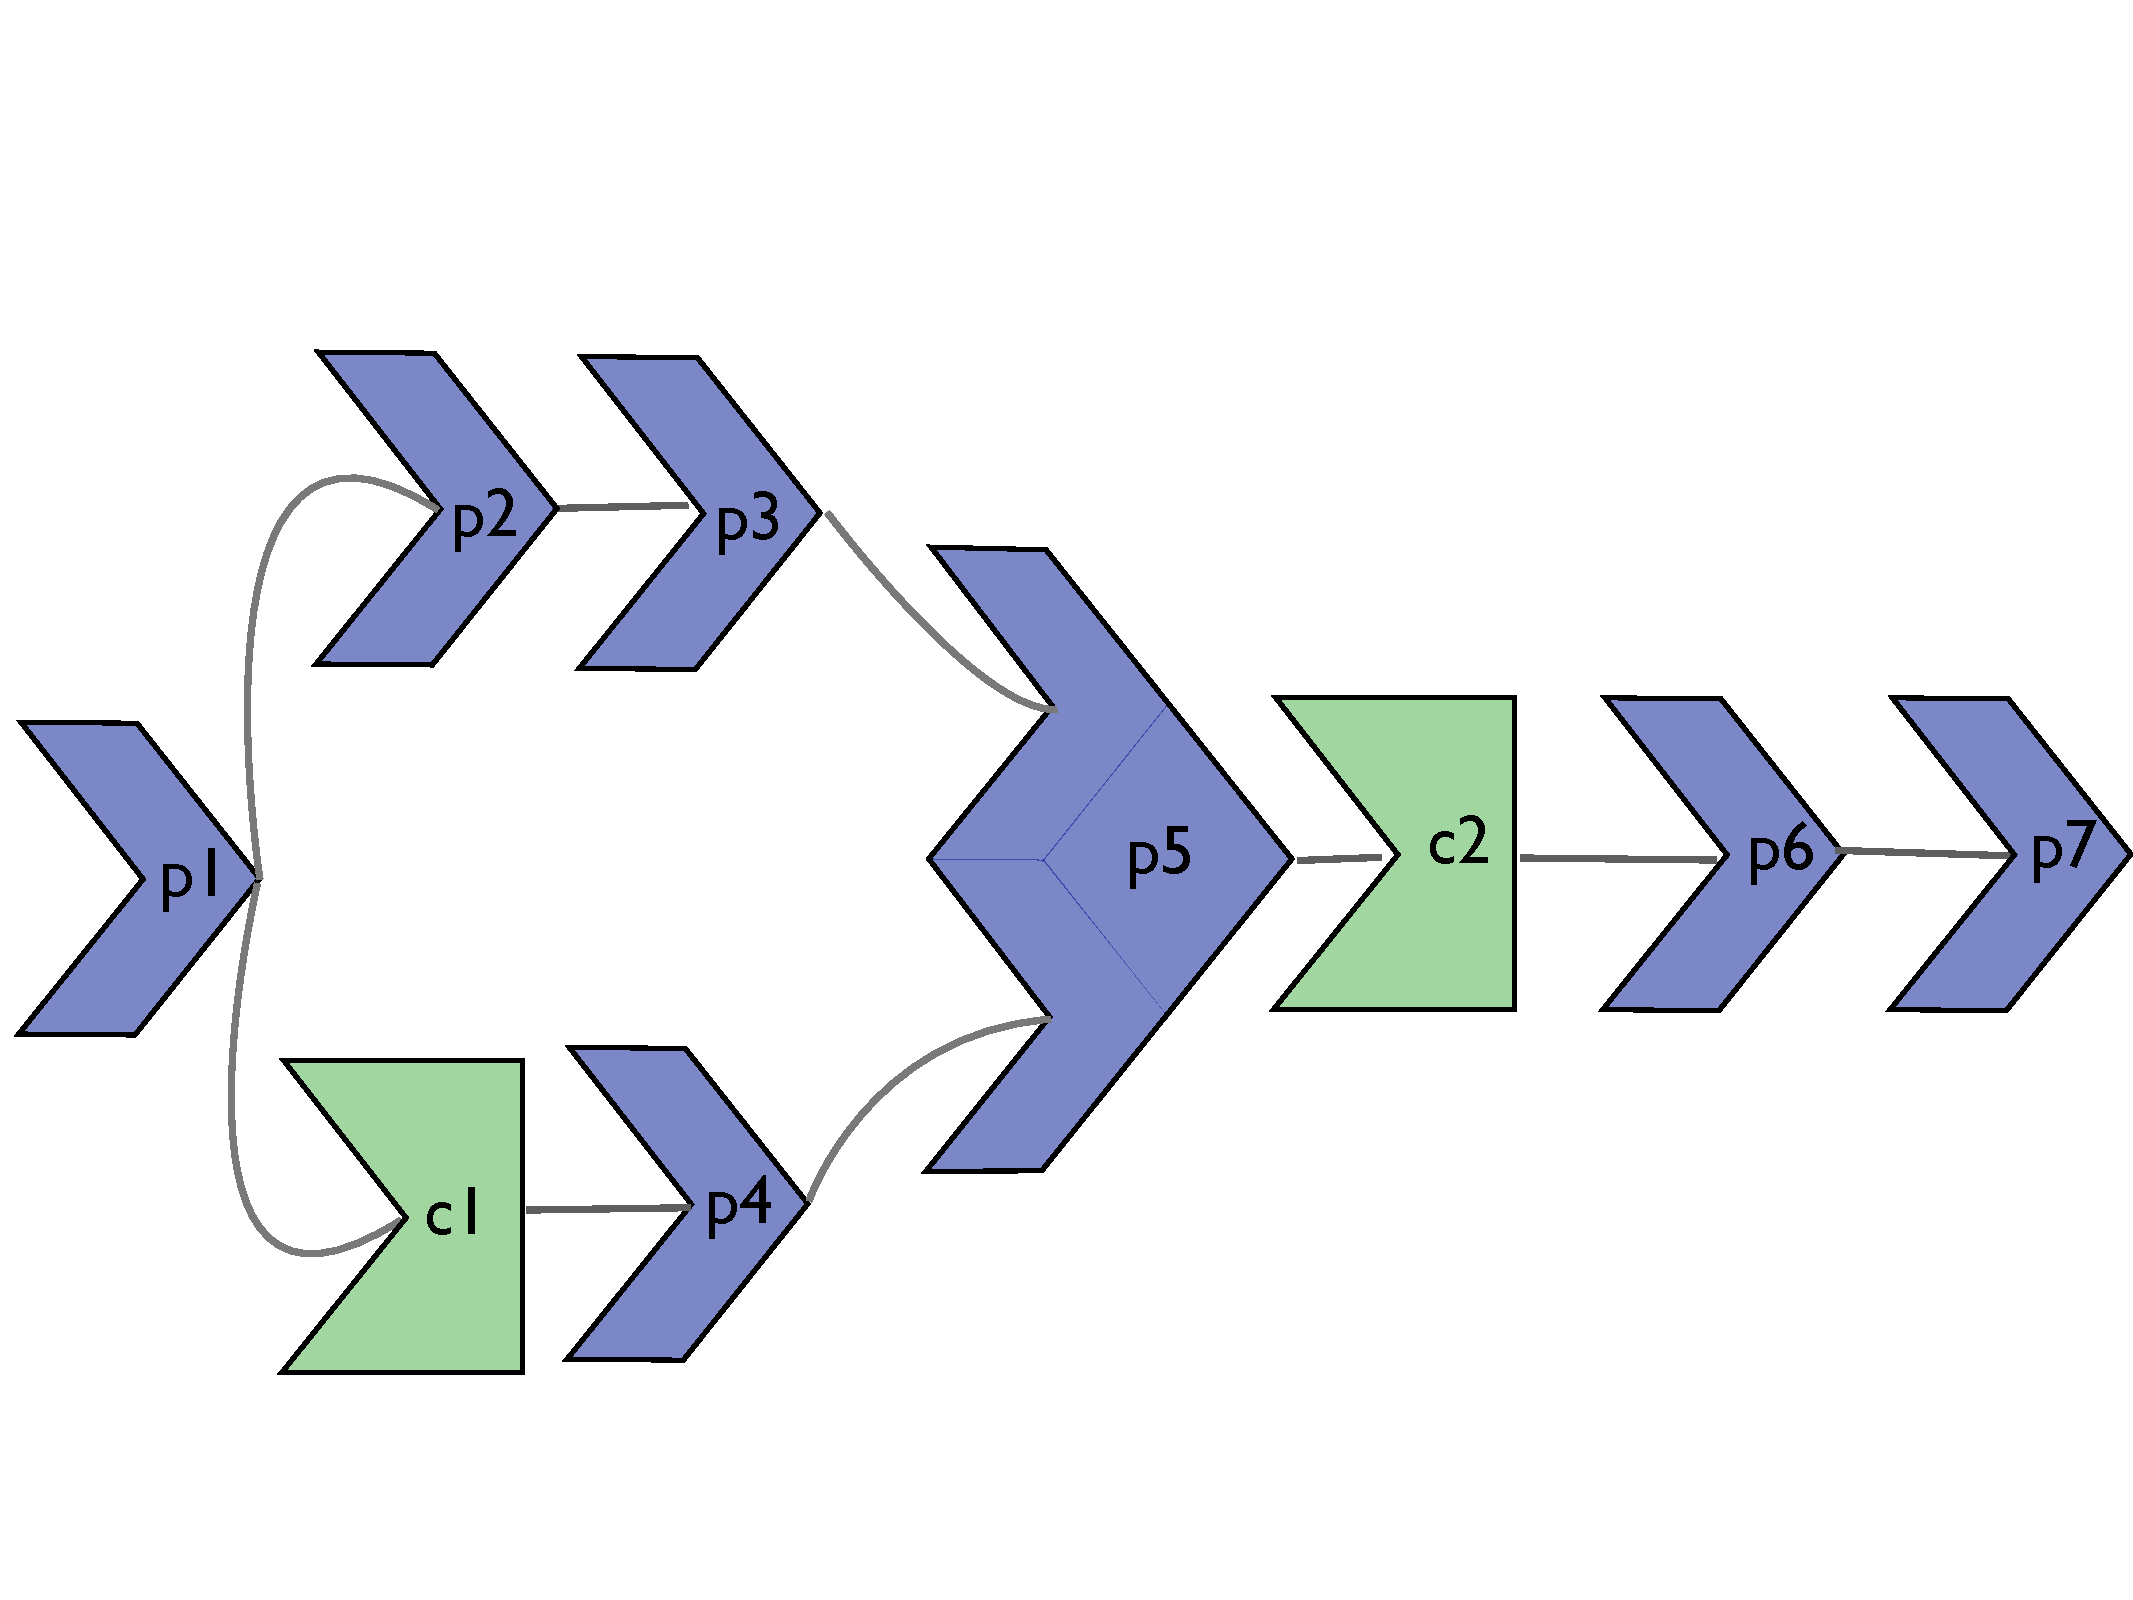
\includegraphics[scale=0.175]{figs/fusion1.pdf}
\flushright
\small(After producer/producer fusion)\qquad\\
\centering
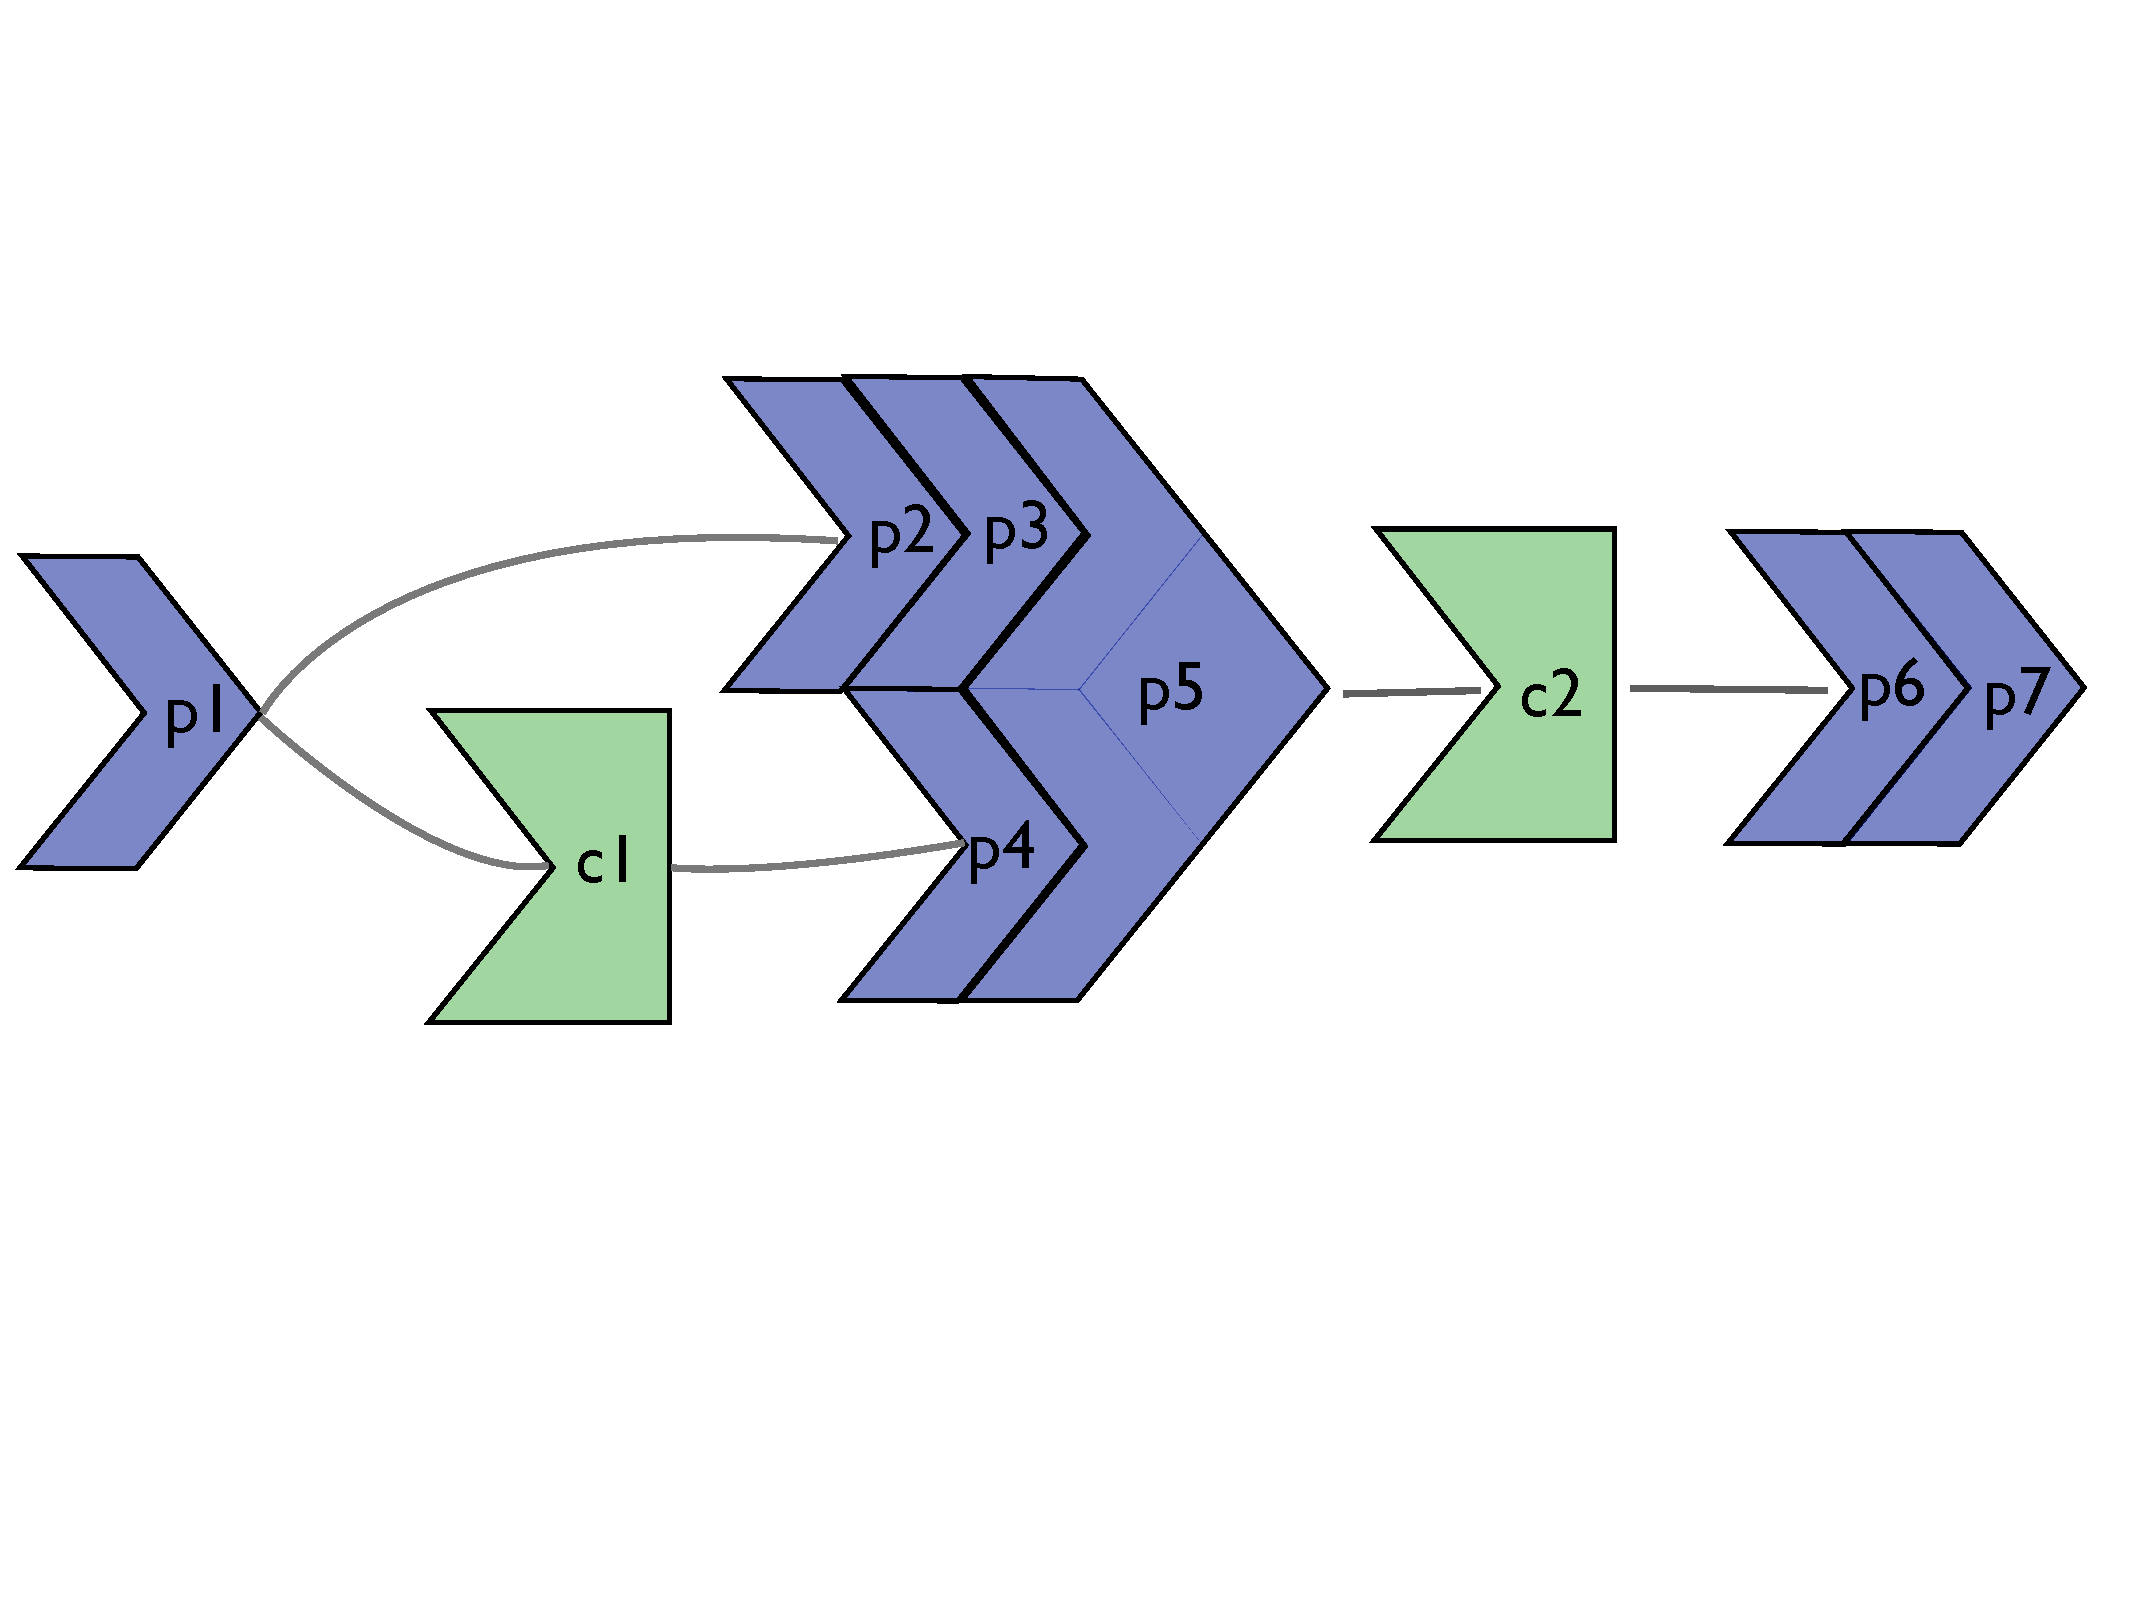
\includegraphics[scale=0.175]{figs/fusion2.pdf}
\flushright
\small(After consumer/producer fusion)\qquad\\
\centering
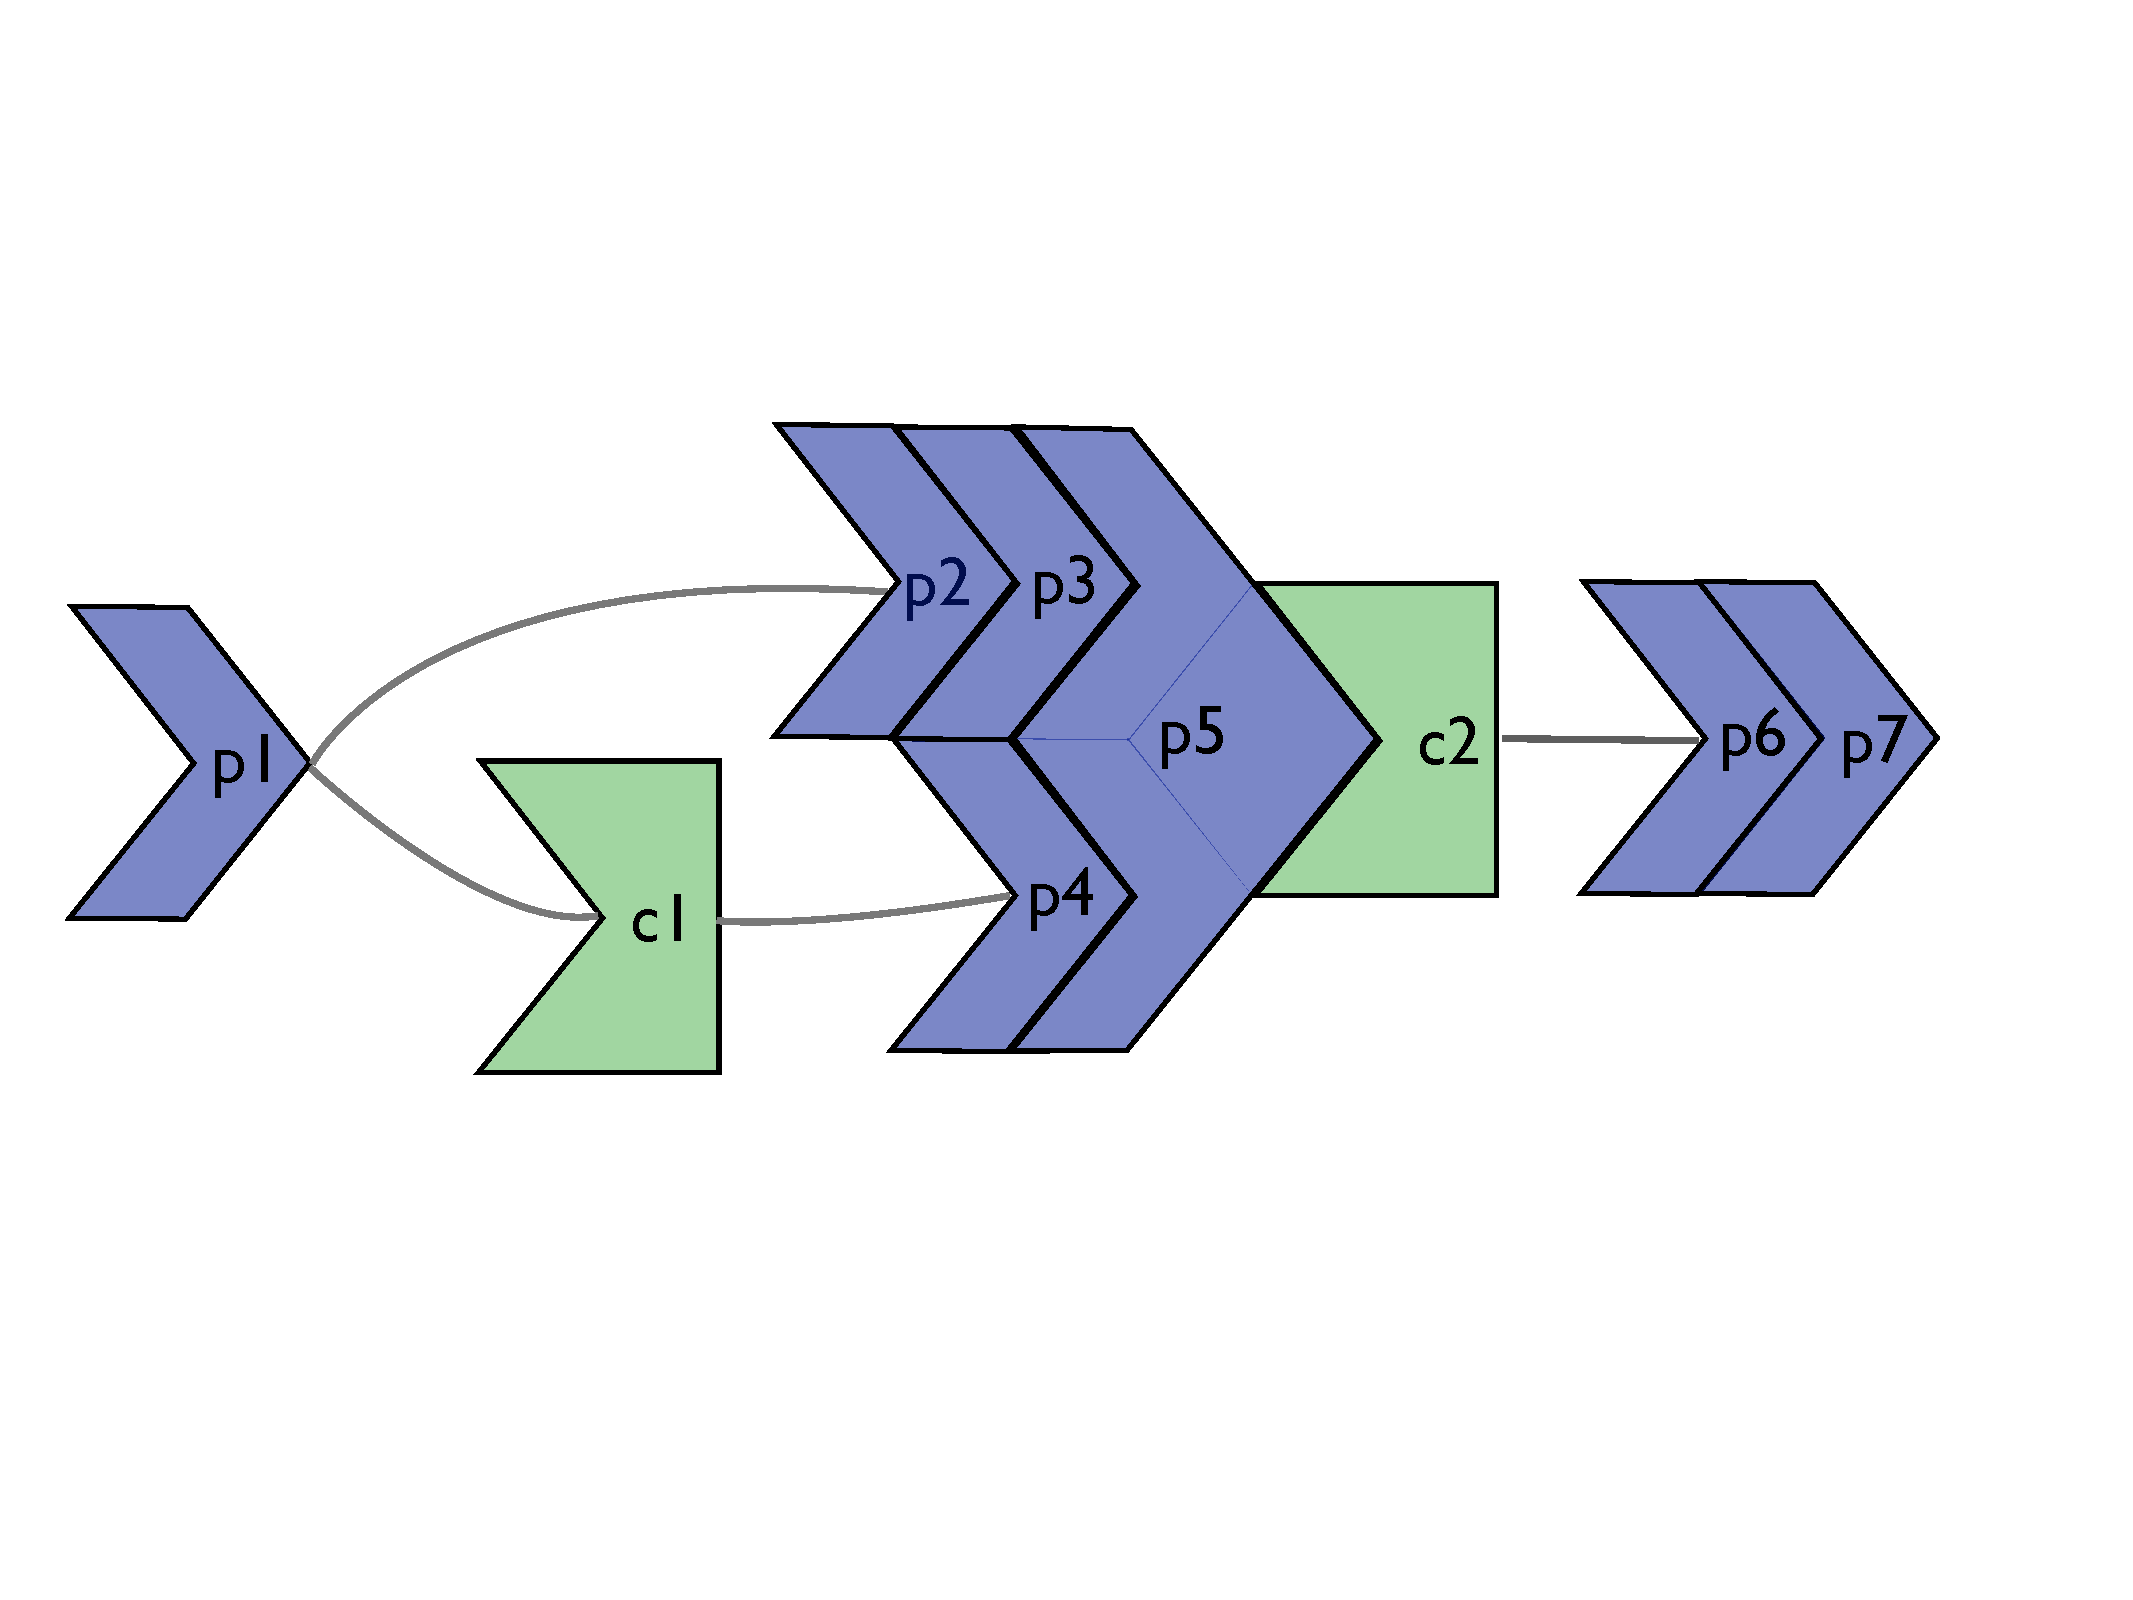
\includegraphics[scale=0.175]{figs/fusion3.pdf}
\caption{Produce/producer and consumer/producer fusion}
\label{fig:Fusion}
\end{figure}

Fusion in a massively data-parallel, embedded language for GPUs, such as Accelerate, requires a few uncommon considerations.

\paragraph{Parallelism.} While fusing parallel collective operations, we must be careful not to lose information essential to parallel execution. For example, \texttt{foldr/build} fusion \cite{Gill:1993de} is not applicable, because it produces sequential tail-recursive loops rather than massively parallel GPU kernels. Similarly, the \texttt{split/join} approach used in Data Parallel Haskell (DPH)~\cite{Keller:distributed-types} is not helpful, although fused operations are split into sequential and parallel subcomputations, as they assume an explicit parallel scheduler, which in DPH is written directly in Haskell. Accelerate compiles massively parallel array combinators to CUDA code via template skeleton instantiation, so any fusion system must preserve the combinator representation of the intermediate code. 

\paragraph{Sharing.} Existing fusion transforms rely on inlining to move producer and consumer expressions next to each other, which allows producer/consumer pairs to be detected. However, when let-bound variables are used multiple times in the body of an expression, unrestrained inlining can lead to duplication of work. Compilers such as GHC, handle this situation by only inlining the definitions of let-bound variables that have a single use site, or by relying on some heuristic about the size of the resulting code to decide what to inline \cite{PeytonJones:Inliner}. However, in typical Accelerate programs, each array is used at least twice: once to access the shape information and once to access the array data; so, we must handle at least this case separately.

\paragraph{Filtering.} General array fusion transforms must deal with filter-like operations, for which the size of the result structure depends on the \emph{value} of the input structure, as well as its size. Accelerate does not encode filtering as a primitive operation, so we do not need to consider it further.\footnote{@filter@ is easily implemented as a combination of the core primitives, and is provided as part of the library.}

\paragraph{Fusion at run-time.}
As the Accelerate language is embedded in Haskell, compilation of the Accelerate program happens at Haskell \emph{runtime} rather than when compiling the Haskell program. For this reason, optimisations applied to an Accelerate program contribute to its overall runtime, so we must be mindful of the cost of analysis and code transformation. On the flip-side, runtime optimisations can make use of information that is only available at runtime. 

\paragraph{Fusion on typed de Brujin terms.}
We fuse Accelerate programs by rewriting typed de Bruijn terms in a type preserving manner. However, maintaining type information adds complexity to the definitions and rules, which amounts to a partial proof of correctness checked by the type checker, but is not particularly exciting for the present exposition. Hence, in this section, we elide the steps necessary to maintain type information during fusion.

\begin{table*}
\begin{lstlisting}[escapechar={\%}]
%\makebox[\textwidth]{\rm\bf Producers}%
map         :: (Exp a -> Exp b) -> Acc (Array sh a) -> Acc (Array sh b)             %\rm map a function over an array%
zipWith     :: (Exp a -> Exp b -> Exp c) -> Acc (Array sh a) -> Acc (Array sh b)    %\rm apply funciton to\ldots%
            -> Acc (Array sh c)                                                     %\rm \ldots a pair of arrays%
backpermute :: Exp sh' -> (Exp sh' -> Exp sh) -> Acc (Array sh a)                   %\rm backwards permutation%
            -> Acc (Array sh' e)
replicate   :: Slice slix => Exp slix                                               %\rm extend array across\ldots%
            -> Acc (Array (SliceShape slix) e)                                      %\rm \ldots new dimensions%
            -> Acc (Array (FullShape  slix) e)
slice       :: Slice slix                                                           %\rm remove existing dimensions%
            => Acc (Array (FullShape  slix) e) -> Exp slix
            -> Acc (Array (SliceShape slix) e)
generate    :: Exp sh -> (Exp sh -> Exp a) -> Acc (Array sh a)                      %\rm array from index mapping%

%\makebox[\textwidth]{\rm\bf Consumers}%
fold        :: (Exp a -> Exp a -> Exp a) -> Exp a -> Acc (Array (sh:.Int) a)        %\rm tree reduction along\ldots%
            -> Acc (Array sh a)                                                     %\rm \ldots innermost dimension%
scan{l,r}   :: (Exp a -> Exp a -> Exp a) -> Exp a -> Acc (Vector a)                 %\rm left-to-right or right-to-left%
            -> Acc (Vector a)                                                       %\rm \ldots vector pre-scan%
permute     :: (Exp a -> Exp a -> Exp a) -> Acc (Array sh' a)                       %\rm forward permutation%
            -> (Exp sh -> Exp sh') -> Acc (Array sh a) -> Acc (Array sh' a)
stencil     :: Stencil sh a stencil => (stencil -> Exp b) -> Boundary a             %\rm map a function with local\ldots%
            -> Acc (Array sh a) -> Acc (Array sh b)                                 %\rm \ldots neighbourhood context%
\end{lstlisting}
\caption[Core Accelerate array operations]{Summary of Accelerate's core
    collective array operations, omitting \texttt{Shape} and \texttt{Elt}
    class constraints for brevity. In addition, there are other flavours of
    folds and scans as well as segmented versions of these.}
\label{tab:operations}
\end{table*}


% -----------------------------------------------------------------------------
\subsection{The Main Idea}
All collective operations in Accelerate are array-to-array transformations. Reductions, such as \texttt{fold}, which reduce an array to a single element, yield a singleton array rather than a scalar expression. Hence, we can partition array operations into two categories:
%
\begin{enumerate}
\item Operations where each element of the result array depends on at most one element of each input array. Multiple elements of the output array may depend on a single input array element, but all output elements can be computed independently. We refer to these operations as \textit{producers}.

\item Operations where each element of the result array depends on multiple elements of the input array. We call these functions \textit{consumers}, in spite of the fact that they also produce an array.
\end{enumerate}
%
Table~\ref{tab:operations} summarises the collective array operations that we support. In a parallel context, producers are more pleasant to deal with because independent element-wise operations have an obvious mapping to the GPU. Consumers are a different story, as we need to know exactly how the computations depend on each other to implement them efficiently. For example, a parallel fold (with an associative operator) can be implemented efficiently as a tree reduction, but a parallel scan requires two separate phases \cite{Sengupta:2007tc, Chatterjee:1990vj}. Unfortunately, this sort of information is obfuscated by most fusion techniques. To support the different properties of producers and consumers, our fusion transform is split into two distinct phases:
%
\begin{itemize}
\item \emph{Producer/producer:} fuse sequences of producers into a single producer. This is implemented as a source-to-source transformation on the AST.

\item \emph{Consumer/producer:} fuse producers followed by a consumer into the consumer. This happens during code generation, where we specialise the consumer skeleton with the producer code.
\end{itemize}
%
Separating fusion into these two phases reduces the complexity of the task, though there is also a drawback: as all collective operations in Accelerate output arrays, we might wish to use the output of a consumer as an input to a producer as in @map g . fold f z@. Here, the \texttt{map} operation could be fused into the \texttt{fold} by applying the function \texttt{g} to each element produced by the reduction before storing the final result in memory. This is useful, as Accelerate works on multidimensional arrays, so the result of a \texttt{fold} can be a large array rather than just a singleton array. Our approach currently does not fuse producer/consumer pairs, only consumer/producer and producer/producer combinations. 

Figure~\ref{fig:Fusion} illustrates how fusion affects the AST: blue boxes $p_1$ to $p_7$ represent producers, where $p_5$ is a producer like \texttt{zipWith} with two input arrays. The consumers are $c_1$ and $c_2$. Firstly, we fuse all producers, with the exception of $p_1$ whose result is used by both $c_1$ and $p_2$. Next, we plug the fused producers into consumers where possible. Again, $p_1$ is left as is. It would be straightforward to change our implementation such that it would fuse $p_1$ into both $p_2$ and $c_1$. This would duplicate the work of $p_1$ into both $p_2$ and $c_1$, which, despite reducing memory traffic, is not always advantageous. Our current implementation is conservative and never duplicates work; we plan to change this in future work as the restricted nature of Accelerate means that we can compute accurate cost estimates and make an informed decision. In contrast, producer/consumer fusion of $c_1$ into $p_4$ would require fundamental changes.


% -----------------------------------------------------------------------------
\subsection{Producer/producer fusion for parallel arrays}

The basic idea behind the representation of producer arrays in Accelerate is well known: simply represent an array by its shape and a function mapping indices to their corresponding values. We previously used it successfully to optimise purely functional array programs in Repa~\cite{Keller:Repa}, but it was also used by others~\cite{Claessen:obsidian-expressive}.

However, there are at least two reasons why it is not always beneficial to represent all array terms uniformly as functions. One is \emph{sharing}: we must be able to represent some terms as manifest arrays so that a delayed-by-default representation can not lead to arbitrary loss of sharing. This is a well known problem in Repa. The other consideration is \emph{efficiency}: since we are targeting an architecture designed for performance, we prefer more specific operations. An opaque indexing function is too general, conveying no information about the pattern in which the underlying array is accessed, and hence no opportunities for optimisation. We shall return to this point in Section~\ref{sec:benchmarks}, but already include a form of structured traversal over an array (@Step@) in the following definition:

% It is parametrised with the shape of the result array, a function which, given
% an index in the result array, returns an index into the manifest source array
% argument.
\begin{code}
  data DelayedAcc a where
    Done  :: Acc a
          -> DelayedAcc a

    Yield :: (Shape sh, Elt e)
          => Exp sh
          -> Fun (sh -> e)
          -> DelayedAcc (Array sh e)

    Step  :: (Shape sh, Shape sh', Elt e, Elt e')
          => Exp sh'
          -> Fun (sh' -> sh)
          -> Fun (e -> e')
          -> Idx (Array sh e)
          -> DelayedAcc (Array sh' e')
\end{code}
%
We have three constructors: \texttt{Done} injects a manifest array into the
type. \texttt{Yield} defines a delayed array in terms of its shape and a
function which maps indices to elements. The third constructor, \texttt{Step},
encodes a special case of the more general \texttt{Yield} that represents the
application of an index and/or value space transformation to the argument array.
The type \texttt{Fun (sh -> e)} is that of a term representing a scalar
function from shape to element type. The type \texttt{Idx (Array sh e)} is that of a de
Bruijn index representing an array valued variable. Representing the argument
array in this way means that both \texttt{Step} and \texttt{Yield} are
non-recursive in \texttt{Acc} terms, and so they can always be expressed as
scalar functions and embedded into consumers in the second phase of fusion.

We represent all array functions as constructors of the type \texttt{DelayedAcc}. Producer/producer fusion is achieved by tree contraction on the AST, merging sequences of producers into a single one. All array producing functions, such as \texttt{map} and \texttt{backpermute}, are expressed in terms of smart constructors for the \texttt{DelayedAcc} type. The smart constructors manage the integration with successive producers, as shown in the following definition of \texttt{mapD}, the delayed version of the \texttt{map} function:
%
\begin{code}
  mapD :: (Shape sh, Elt a, Elt b)
       => Fun (a -> b)
       -> DelayedAcc (Array sh a)
       -> DelayedAcc (Array sh b)
  mapD f (Step  sh p g v) = Step  sh p (f . g) v
  mapD f (Yield sh g)     = Yield sh   (f . g)
\end{code}
%
The function composition operator \texttt{(.)} is overloaded here to work on scalar function terms. With this definition we now have the well known fusion rule that reduces \texttt{mapD f . mapD g} sequences to \texttt{mapD (f . g)}. Similarly, the definition of delayed backpermute means that \mbox{\texttt{backpermuteD sh p (backpermuteD \_ q arr)}} reduces to \texttt{backpermute sh (q . p) arr}:
\begin{code}
backpermuteD
    :: (Shape sh, Shape sh', Elt e)
    => Exp        sh'
    -> Fun        (sh' -> sh)
    -> DelayedAcc (Array sh  e)
    -> DelayedAcc (Array sh' e)
backpermuteD sh' p acc = case acc of
  Step  _ ix f a  -> Step  sh' (ix . p) f a
  Yield _ f       -> Yield env sh' (f . p)
  Done  env a     -> Step  sh' p identity (toIdx a)
\end{code}
% \gck{Manuel: as discussed, we may have to put in the valuation. Does backpermute really add anything here anyway?}
Of course, combinations of maps with backpermutes also reduce to a single producer. %, albeit one that does not correspond to one of the Accelerate built-in array operations.

As desired, this approach also works on producers which\linebreak
take their input from multiple arrays. This is in contrast to\linebreak
\texttt{foldr/build}~\cite{Gill:1993de}, which
can fuse one of the input arguments, but not both. The definition of \texttt{zipWithD} considers 
all possible combinations of constructors (only some of which we list here) and can therefore fuse producers of both arguments:
%
\begin{code}
  zipWithD :: (Shape sh, Elt a, Elt b, Elt c)
           => Fun (a -> b -> c)
           -> DelayedAcc (Array sh a)
           -> DelayedAcc (Array sh b)
           -> DelayedAcc (Array sh c)
  zipWithD f (Yield sh1 g1) (Yield sh2 g2)
    = Yield (sh1 `intersect` sh2)
            (\sh -> f (g1 sh) (g2 sh))
  zipWithD f (Yield sh1 g1) (Step  sh2 ix2 g2 a2)
    = Yield ...
\end{code}
%
In this manner, sequences of producers fuse into a single producer term; then, we turn them back into a manifest array using the function \texttt{compute}. It inspects the argument terms of the delayed array to identify special cases, such as maps or backpermutes, as shown in the following snippet of pseudo-code:
%
\begin{code}
  compute :: DelayedAcc a -> Acc a
  compute (Done a)          = a
  compute (Yield sh f)      = Generate sh f
  compute (Step sh p f v)
    | sh == shape a, isId p, isId f 
                            = a
    | sh == shape a, isId p = Map f a
    | isId f                = Backpermute sh p a
    | otherwise             = Transform sh p f a
    where a = Avar v
\end{code}
%
Since we operate directly on the AST of the program, we can inspect function arguments and specialise the code accordingly. For example, \texttt{isId :: Fun (a->b) -> Bool} checks whether a function term corresponds to the term $\lambda x. x$. 


% -----------------------------------------------------------------------------
\subsection{Consumer/Producer Fusion}
Now that we have the story for producer/producer fusion, we discuss how to deal with consumers. We pass producers encoded in the @DelayedAcc@ representation as arguments to consumers, so that the consumers can compute the elements they need on-the-fly. Consumers themselves have no @DelayedAcc@ representation, however.

Consumers such as \texttt{stencil}, access elements of their argument array multiple times. These consumers are implemented carefully not to duplicate work. Indeed, even when the argument of such a consumer is a manifest array, the consumer should ensure that it caches already fetched elements, as GPUs impose a high performance penalty for repeated memory loads. Some consumers can be implemented more efficiently when given a producer expressed in terms of a function from a multi-dimensional array index to an element value. Other consumers prefer functions that map the flat linear index of the underling array to its value. Our consumer-friendly representation of delayed arrays therefore contains both versions: 
%
\begin{code}
data Embedded sh e
  =  (Shape sh, Elt e) 
  => DelayedArray { extent      :: Exp sh
                  , index       :: Fun (sh  -> e)
                  , linearIndex :: Fun (Int -> e) }

embedAcc :: (Shape sh, Elt e) 
         => Acc (Array sh e) -> Embedded sh e
embedAcc (Generate sh f)  
  = DelayedArray sh f (f . (fromIndex sh))
embedAcc (Map f (AVar v)) 
  = DelayedArray (shape v) (indexArray v) 
                           (linearIndexArray v)
embedAcc ...
\end{code}
%
The function \texttt{embedAcc} intelligently injects each producer into the \texttt{Embedded} type by inspection of the constructor, as shown in the code snippet above. In theory, \texttt{compute} and \texttt{embedAcc} could be combined to go directly from the delayed representation which is convenient for producer/producer fusion to the one for consumer/producer fusion. However, these two steps happen at different phases in the compilation, so we want to limit the visibility of each delayed representation to the current phase.

Producers are finally embedded into consumers during code generation. During code generation, the code for the embedded producers is plugged into the consumer template. The \texttt{codegenAcc} function inspects the consumer and generates code for the arguments of the consumer. It then passes these CUDA code snippets to a function specialised on generating code for this particular consumer (\texttt{mkFold} in the example below), which combines these snippets with the actual CUDA consumer code:
\begin{code}
 codegenAcc :: DeviceProperties -> OpenAcc arrs 
            -> Gamma aenv -> CUTranslSkel arrs 
 codegenAcc dev (OpenAcc (Fold f z a)) aenv 
   = mkFold dev  aenv (codeGenFun f) (codeGenExp z) 
            (codegenDelayedAcc $ embedAcc a)
 codegenAcc dev (OpenAcc (Scanl f z a)) aenv 
   = ...
\end{code}
%
As a result, the code producing each element is integrated directly into the consumer, and no intermediate array needs to be created.


% -----------------------------------------------------------------------------
\subsection{Exploiting all opportunities for fusion}

As mentioned previously, we need to be careful about fusing shared array computations, to avoid duplicating work. However, \emph{scalar} Accelerate computations that manipulate \emph{array shapes}, as opposed to the bulk array data, can lead to terms that employ sharing, but can never duplicate work. Such terms are common in Accelerate code, and it is important to that they do not inhibit fusion.

Consider the following example that first reverses a vector with @backpermute@ and then maps a function @f@ over the result. Being a sequence of two producer operations, we would hope these are fused into a single operation:
%
\begin{code}
  reverseMap f a
    = map f
    $ backpermute (shape a) (\i->length a-i-1) a
\end{code}
%
Unfortunately, sharing recovery, using the algorithm from Section~\ref{sec:sharing}, causes a problem. The variable @a@ is used three times in the arguments to @backpermute@; hence, sharing recovery will introduce a let binding at the lowest common meet point for all uses of the array. This places it between the \texttt{map} and \texttt{backpermute} functions:
%
\begin{code}
  reverseMap f a
    = map f
    $ let v = a
      in backpermute (shape v) (\i->length v-i-1) v
\end{code}
%
This binding, although trivial, prevents fusion of the two producers, and it does so unnecessarily. The argument array is used three times: twice to access shape information, but only once to access the array data --- in the final argument to \texttt{backpermute}. 

Fortunately, there is a simple work around. Recall that our delayed array constructors \texttt{Step} and \texttt{Yield} carry the shape of the arrays they represent. Hence, we can eliminate all uses of the array that \emph{only access shape information}, leaving us with a single reference to the array's payload. That single reference enables us to remove the let binding and to re-enable fusion.

Similarly, we may float let bindings of manifest data out (across producer chains). This helps to expose further opportunities for producer/producer fusion. For example, we allow the binding of \texttt{xs} to float above the \texttt{map} so the two producers can be fused:
%
\begin{code}
  map g $ let xs = use (Array ...)
          in zipWith f xs xs
\end{code}

While floating let bindings opens up the potential for further optimisations, we are careful to not increase the lifetime of bound variables, as this would increase live memory usage.


% % -----------------------------------------------------------------------------
% \subsection{Hylomorphism Fusion}
% On a denotational level, our array fusion system is an instance of hylomorphism fusion as described by Takano and Meijer in \cite{Takano:shortcut-calculational}. Recall from \cite{Meijer:bananas} that a hylomorphism is a combination of an \emph{anamorphism} (unfold) that creates a bulk structure, followed by a \emph{catamorphism} (fold) that immediately reduces it. In \cite{Takano:shortcut-calculational} the ``bulk structures'' are presented as general F-algebras, and a third component gives a natural transformation between the input and output algebras. For the present discussion we can think of an F-algebra as an abstract data type, though see \cite{Takano:shortcut-calculational} for the formal definition. The three components of a hylomorphism are bundled together in ``envelope'' brackets which have the following signature.
% $$
% [\_, \_, \_]_{G,F} 
%         : \forall A B
%         . (G A \to A) \times (F \to G) \times (B \to F B)
%         \to (B \to A)
% $$

% For a given hylomorphism $[\varphi, \eta, \psi]$ the $\varphi$ is the catamorphism (fold) part, $\eta$ is the natural transformation, and $\psi$ is the anamorphism (unfold) part. 

% The @foldGen@ function described in \REF allows us to evaluated a restricted form of hylomorphism, namely one that can be efficiently computed on our parallel machine. 

% \begin{code}
%   foldGen :: Exp (sh :. Int) 
%           -> Fun ((sh :. Int) -> e)
%           -> Fun (e -> e -> e) 
%           -> Exp e 
%           -> Acc (Array sh e)
% \end{code}

% In @foldGen@, the first two arguments define the anamorphism (unfold), and the last two give the catamorphism (fold). Whereas the formal system of \cite{Takano:shortcut-calculational} expresses fusion over arbitrary data types, Accelerate only works on parallel arrays. In regards to the general definition, $B$ corresponds to array index @(sh :. Int)@ and $A$ corresponds to the result value @(Array sh e)@. The two functors $F$ and $G$ are fixed by the implementation. The object $F B$ is the function that takes each index and produces the element at that index @((sh:.Int) -> e)@. The object $G A$ corresponds to the intermediate array @(Array (sh:.Int) e)@ before it is reduced to @(Array sh e)@. The natural transformation performs the representation change between the two ``views'' of the intermediate array, that of a function that produces elements @((sh:.Int) -> e)@, and that of an indexable data structure @Array (sh:.Int) e@. The producer and consumer rules of \REF are then instances of the Cata-Hylo and Hylo-Ana fusion rules of   \cite{Takano:shortcut-calculational}.


% % -----------------------------------------------------------------------------
% \subsection{Hylomorphism fusion for parallel arrays}
% ... compare our instance of the anamorphism so the one from the standard Haskell library:

% @unfoldr :: (s -> (s, a)) -> s -> List a@

% In this case underlying functor $F$ provides a state parameter @s@ that is threaded through the computation. Although the state parameter allows the value of each successive element to depend on the previous one, it also makes the computation naturally sequential, so is not appropriate for our purposes.

% \ben{Say something about how @foldGen@ changes the index space from @(sh :. Int)@ to plain @sh@}.

% section fusion (end)

%!TEX root = ../Main.tex
\clearpage{}
\section{Benchmarks}

\begin{figure}
\begin{code}

\end{code}
\caption{Analytic Operators}
\end{figure}

%!TEX root = ../acc-optim.tex
\section{Related work} % (fold)
\label{sec:related}
Repa \cite{Keller:Repa} is a Haskell library for parallel array programming on shared-memory SMP machines. Repa uses the \mbox{delayed/manifest} representation split on which our @DelayedAcc@ type is based, though the idea of representing arrays as functions is folklore. With Repa the conversion between array representations is done manually and can cause shared expressions to be recomputed rather than stored. Such recomputation can improve runtime performance depending on the algorithm. In Accelerate the conversion is automatic and conservative, so that shared expressions are never recomputed. 

Vertigo~\cite{Elliott:Vertigo}, Nikola \cite{Mainland:nikola} and Obsidian \cite{Claessen:obsidian} are EDSLs in Haskell and were mentioned in Section~\ref{sec:Introduction}. Vertigo is a first-order language for writing shaders, and does not provide higher-order combinators such as @map@ and @fold@. Nikola uses an instance of Gill's approach~\cite{Gill:2009dx} to sharing recovery, is limited to single GPU kernel programs, and performs no fusion. 

Obsidian~\cite{Claessen:obsidian} is a lower level language where more details of the GPU hardware are exposed to the programmer. Recent versions of Obsidian \cite{Claessen:obsidian-expressive} implement Repa-style delayed \emph{pull arrays} as well as \emph{push arrays}. Whereas a pull array represents a general producer, a push array represents a general consumer. Push arrays allow the intermediate program to be written in continuation passing style (CPS), and helps to compile (and fuse) append-like operations.

Baracuda~\cite{Larsen:baracuda} is another Haskell EDSL that produces CUDA GPU kernels, though is intended to be used offline, with the kernels being called directly from C++. The paper~\cite{Larsen:baracuda} mentions a fusion system that appears to be based on pull arrays, though the mechanism is not discussed in detail. Barracuda steps around the sharing problem by requiring let-bindings to be written using the AST node constructor, rather than using Haskell's native let-expressions.

Delite/LMS~\cite{Rompf-etal:Delite} is a parallelisation framework for DSLs in Scala that uses library-based multi-pass staging to specify complex optimisations in a modular manner. Delite supports loop fusion for DSLs targeting GPUs using rewrite rules on a graph-based IR.

NDP2GPU~\cite{bergstrom:ndp2gpu} compiles NESL code down to CUDA. As the source language is not embedded there is no need for sharing recovery. NDP2GPU performs @map@/@map@ fusion but cannot fuse @map@s into reduction combinators.

Sato and Iwasaki~\cite{Sato:Skeletal-fusion} describe a C++ library for GPGPU programming that includes a fusion mechanism based on list homomorphisms~\cite{Meijer:bananas}. The fusion transformation itself is implemented as a source to source translation. SkeTo \cite{Matsuzaki:Skeletal-expression-templates} is a C++ library that provides parallel skeletons for CPUs. SkeTo's use of C++ templates provides a fusion system similar to delayed arrays, which could be equivalently implemented using CUDA templates. The authors of SkeTo note that the lack of type inference in C++ leads them to write their array code as nested expressions --- to avoid intermediate variable bindings and their required type annotations.

% section related (end)

%!TEX root = ../acc-optim.tex
% \section{Conclusions} % (fold)
% \label{sec:Conclusions}
% \TODO{Summarise where we're at with the benchmarks. What still needs to be improved.}


% section Conclusions (end)


\paragraph{Acknowledgements.}
This work was supported in part by the Australian Research Council under grant number LP0989507.

% ------------------------------------------------------------------------------
\bibliographystyle{abbrvnat}
\bibliography{acc-optim}


\end{document}

